\documentclass[sigconf]{acmart}
\usepackage{listings}
\usepackage{hyperref}
\begin{document}

\title{Pennant Lines: An Alternative to Finger Trees in Dynamic Environments}

\author{Daniel Jay Haskin}

\acmConference[ELS '25]{European Lisp Symposium}{May 15--23,
  2025}{Vienna, Austria}
\email{dan@djhaskin.com}
\renewcommand{\shortauthors}{Haskin}

\begin{abstract}
Pennant Lines are presented, a novel data structure for storing persistent
sequences in Common Lisp suitable as a drop-in replacement for normal lists, but
with much better runtimes for most operations. These sequences support at least
logarithmic time when implementing a version of the Common Lisp Sequences API
persistently, and better time in other key cases. All are simpler to implement
within a dynamic setting such as that of Common Lisp than Finger Trees, and play
nicer with the larger Lisp ecosystem.
\end{abstract}

%% https://dl.acm.org/ccs.cfm
\begin{CCSXML}
<ccs2012>
<concept>
<concept_id>10003752.10003809.10010031</concept_id>
<concept_desc>Theory of computation~Data structures design and analysis</concept_desc>
<concept_significance>500</concept_significance>
</concept>
</ccs2012>
\end{CCSXML}
\ccsdesc[500]{Theory of computation~Data structures design and analysis}
\keywords{lisp, datastructure, sequences, dynamic, untyped}

%%\begin{teaserfigure}
%%  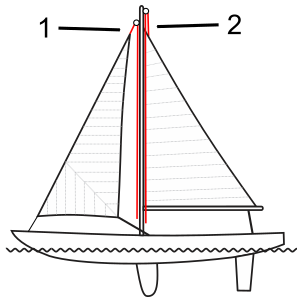
\includegraphics[width=\textwidth]{img/Halyard}
%%  \caption{A depiction of a Halyard[1].}
%%  \Description{A drawing of a sailbosat with the main and jib halyards
%%    highlighted.}
%%  \label{fig:teaser}
%%\end{teaserfigure}

%%\received{20 February 2007}
%%\received[revised]{12 March 2009}
%%\received[accepted]{5 June 2009}
\maketitle

\section{Motivation}

When in a dynamically typed language like Lisp, it is often convenient to work
with a data structure in specific ways in one moment, such as for operating on
sets, and then perform simple list operations on them the next. Alists are nice
because at the end of the day, "they are just lists" -- they can be fed into
functions that expect an array of items, like \texttt{print}. Object type is
fluid in Lisp, as is object purpose. In Lisp, data structures can be used for
their characteristics and ergonomics, rather than for their intended type. Lisp
is a highly dynamic environment.

In the dynamic environment of Common Lisp, lists are used for
\emph{everything}, from dictionaries to sets to arrays. All the tooling works
better with these data structures than with anything else. Getting the nth
element, performing set union or intersection, stack operations, and syntax
abstractions on lists are all defined in the Common Lisp standard.

However, lists present poor run time characteristics when used for anything more
complicated than a stack. Often lists are used simply because of their ease of
use with little regard for runtime. This is fine until the runtime becomes
important; then ergonomics is sacrificed and the code is rewritten data
structures which are faster, but less ergonomic.

In this presentation, we will implement a data structure with an API that imitates
the Common Lisp list API but in a way that is ergonomic, persistent by default,
and dynamic. This means the resulting data structure must be usable as a list
first, but sometimes also as a set or dictionary. By implementing functions
that mirror the list API, we make it easy for people to use the structure, since
all the functions they are used to using with lists exist and work just as they
do for lists, they just exist in a different package.

As a first attempt at this task, Finger Trees \cite{Hinze-Paterson:FingerTree}
were first examined. Finger Trees are easy
to implement in Haskell, with its algebraic sum types and pattern matching. The
problem is that they are clunky to implement in a dynamically typed language
like Lisp. Implementing Finger Trees involves polymorphic recursion. Every level
in a finger tree contains deeper 2-3 trees than the level above it, and values
are only at the leaves. The spine of the tree is different than the leaves.

This creates a lot of case-by-case work in Lisp. The CLOS is well designed, but
can be slow, especially in the "hot path" in which data structure operations
often find themselves. Without using the CLOS, we are left with the choice of
using \texttt{defstruct} and \texttt{typecase}, both of which greatly complicate
the implementation.

It would be ideal if the data structure were relatively homogeneous -- it looked
the same throughout. This would greatly decrease case logic.
%% We also want structure that is cons-based. That way, it is still "just a list"
%% and can work with a lot of list tooling --
%$% \texttt{destructuring-bind}, \texttt{copy-tree}, \texttt{tree-equal},
%% \texttt{print}, etc.

Finally, we need a structure that is tolerant to and implements functionality
for non-persistent updates along side the persistent ones. This mirrors how
lists are used in Common Lisp -- persistent by default, but changeable if need
be.

So, we need to create a data structure that is relatively homogeneous, with
few cases to manage. It must be able to be used dynamically for different
purposes. It must be persistent by default, but changeable if needed. It should
have good running time. Finally, its API should closely mirror the Common Lisp
Standard's List API.

\section{Development}

In this section we first lay out the API that needs to be implemented and summarize
what functionality needs to exist for that API. We then develop an answer to
that API with weight-balanced binary trees. Finally, develop even better run
times by adding pennant lines to the mix.

\subsection{The List API}

The Common Lisp Standard's API for lists\cite{ANSI:1994:DPA} outlines three
basic uses for conses (among others):

\begin{enumerate}
    \item As sequences of items (speaking of "proper lists").
    \item As association structures.
    \item As sets.
\end{enumerate}

We will also seek to make a datastructure suitable for these three uses using a
persistent-by-default structure. Therefore, the following operations need to be
supported:

\begin{itemize}
    \item Efficient random insertion, deletion, and access, particularly at the
        ends
    \item Efficient reduction (using a \texttt{reduce}-like function)
    \item Efficient concatenation
    \item Efficient splitting / subsequencing
    \item Efficient set operations
\end{itemize}

These will be used separately or in combination depending on the API function in
which it is used.

Then we implement the API on top of these basic operations, which will support
sets, associative structures, and plain sequences of objects.

\subsection{Observations about Ranked Binary Trees}

We first note that the Hinze and Paterson's Finger Tree ``monoid
trick''\cite{Hinze-Paterson:FingerTree} can actually be done with any tree,
including a binary search tree.

\begin{lstlisting}[caption={Our indexed binary tree type.}, label={lst:treestruct}, language=Lisp]
;;; Indexed node within a binary tree.
(defstruct node
    value
    size
    left
    right)
\end{lstlisting}

Throughout the rest of this paper, when discussing binary trees, we will use
the definition in listing \ref{lst:treestruct}.

Suppose each node in a binary search tree has also a `size` component. Then,
provided an index into the tree, insert, delete, and access operations can
be done without comparing values in the tree to each other by instead comparing
tree and subtree sizes to the currently given index. In this way, a value
can be inserted, deleted, or accessed at the given index in logarithmic time.

The access algorithm is straightforward. The index is compared against the size
components of the left and right child of the root. If the left child's size
is greater than the index, insertion recurses into the left child using the same
index. If the index equals the left child size, the value of the root node is returned.
If it is greater than the left child size, insertion recurses into the right
child using \texttt{(- index 1 (node-size (node-left tree)))} as the index.

Insertion works by finding the indexed node, swapping the value at that spot
with the value that needs inserted, and then recursing into the right child with
the swapped out value and an index of 0, followed by a rebalancing step going
back up the tree.

Deletion works by finding the indexed node, deleting the value at that spot,
then, deleting the value from the right child at index 0 (or the left child at
index \texttt{(-1 (node-size left-child))} and placing that value in the spot
which we leave behind, rebalancing as we go.

That gives us a logarithmic baseline for insertion, random access, deletion and
stack-based traversal. We still need concatenation, splitting, and set
operations. For concatenation and splitting, we can use the work due to Guy E.
Blelloch, Daniel Ferizovic, and Yihan Sun\cite{10.1145/3512769}. We'll also use
their work a bit later for set operations\cite{DBLP:journals/corr/BlellochFS16}.

We choose, then, to use "normal" binary trees as the
basis of our new data structure, instead of 2-3 leaf trees. That way, the data
structure is much more homogeneous; the code becomes simpler, with fewer cases.

Binary trees will give us a nice baseline of logarithmic time for many
operations, but if we want efficient insertion at the beginning and end, we will
have to use a Zipper\cite{HUET_1997}, kind of like Hinze and
Patterson\cite{Hinze-Paterson:FingerTree} did with Finger Trees. That means
there will be added polymorphism and hence complexity, but it will not be too
much.


\subsection{Sorted Mode: Speeding Up Set Operations}

Binary trees are a good basis for our use case for another reason: there's
nothing stopping us from treating these trees as "normal sorted sets" like the
ones that are customarily kept inside trees (rather than sequences). Operating
in a different mode on the same data structure, we could treat these "sequences"
like sets, or these "sets" like sequences. In one mode, we insert by index; in
another mode, we insert using a sort function that finds its way through the
tree by comparing the given value to insert with its compatriots in the tree.
This information could be given at runtime, using a \texttt{:sortfn <fn>}
argument instead of an \texttt{:index <ind>} to one of our functions that
operate on these pennants. Indexed binary search trees can be treated as a
set or a sequence fluidly.

When we insert, we provide a sort function instead of an index, and say that
$<=$ is used for inserting into the left child instead of $<$, now we just have
a "normal" multiset that can be merged using Guy Blelloch's stuff. We could
also take an unsorted thing and run `sort` on it and that gives a new sequence
that's sorted and immediately usable in "sorted mode".

Further, if a \texttt{:sortfn <fn>} were given to some e.g. set operation
function in our API, and was used throughout the life of the data structure, we
could then treat the tree like an ordered set and use the set operations
provided in \cite{DBLP:journals/corr/BlellochFS16} instead of treating the trees
like fancy lists when implementing the set operations. If \texttt{:sortfn}
parameter is not given, we may assume the tree is unordered, and we will just
treat the trees like normal unordered sequences when performing set operations.

\subsection{Picking the Binary Tree Balancing Algorithm}

We have one more detail to add before our baseline can be complete, though. We
must select a balancing algorithm for the tree.

We select weight balanced trees. Weight-balanced trees were originally presented
due to J. Nievergelt and E. M. Reingold\cite{doi:10.1137/0202005}, but most
recently to Y. Hirai and K. Yamamoto\cite{HIRAI_YAMAMOTO_2011}. The advantage of
weight balanced trees is that height of the trees are kept track using the size
element, something the design already requires.

The drawback is that height is
roughly kept track of effectively using the most significant bit of the size of
the tree. Thus, the ``taller'' the tree, the more bits are needed to represent
size and overflows may occur. This is fine though, since we're in Common Lisp,
since its numerical tower prevents all of that. Also, a tree of height e.g. 50
is of roughly of size $2^48$ to $2^52$ with Hirai and Yamamoto's $<3,2>$ Weight
Balanced Trees. This is both large enough to have few if any applications, but
it is also small enough to fit in the mantissa of a 64-bit floating point
integer. This means this strategy would work in most places, even in
math-constrained ones like Janet\cite{Janet} or JavaScript.

The other disadvantage is that integer multiplication is needed to get weights
to balance, but with the parameters given by Hirai and Yamamoto it is a simple
arithmetic shift followed by an addition (multiply by $3$) for $\Delta$ and a
simple arithmetic shift for $\Gamma$, so that's not a problem either. (In 64-bit
float languages, it's an increment of the exponent and addition or simply
exponent increment, and is equally easy to do.)

(Draft note, primer for WB trees goes here in the actual paper)

\section{Tables}


Immediately following this sentence is the point at which
Table~\ref{tab:freq} is included in the input file; compare the
placement of the table here with the table in the printed output of
this document.

\begin{table}
  \caption{Frequency of Special Characters}
  \label{tab:freq}
  \begin{tabular}{ccl}
    \toprule
    Non-English or Math&Frequency&Comments\\
    \midrule
    \O & 1 in 1,000& For Swedish names\\
    $\pi$ & 1 in 5& Common in math\\
    \$ & 4 in 5 & Used in business\\
    $\Psi^2_1$ & 1 in 40,000& Unexplained usage\\
  \bottomrule
\end{tabular}
\end{table}

To set a wider table, which takes up the whole width of the page's
live area, use the environment \textbf{table*} to enclose the table's
contents and the table caption.  As with a single-column table, this
wide table will \texttt{''float} to a location deemed more
desirable. Immediately following this sentence is the point at which
Table~\ref{tab:commands} is included in the input file; again, it is
instructive to compare the placement of the table here with the table
in the printed output of this document.

\begin{table*}
  \caption{Some Typical Commands}
  \label{tab:commands}
  \begin{tabular}{ccl}
    \toprule
    Command &A Number & Comments\\
    \midrule
    \texttt{{\char'134}author} & 100& Author \\
    \texttt{{\char'134}table}& 300 & For tables\\
    \texttt{{\char'134}table*}& 400& For wider tables\\
    \bottomrule
  \end{tabular}
\end{table*}

Always use midrule to separate table header rows from data rows, and
use it only for this purpose. This enables assistive technologies to
recognise table headers and support their users in navigating tables
more easily.

\section{Math Equations}
You may want to display math equations in three distinct styles:
inline, numbered or non-numbered display.  Each of the three are
discussed in the next sections.

\subsection{Inline (In-text) Equations}
A formula that appears in the running text is called an inline or
in-text formula.  It is produced by the \textbf{math} environment,
which can be invoked with the usual
\texttt{{\char'134}begin\,\ldots{\char'134}end} construction or with
the short form \texttt{\$\,\ldots\$}. You can use any of the symbols
and structures, from $\alpha$ to $\omega$, available in
\LaTeX~\cite{Lamport:LaTeX}; this section will simply show a few
examples of in-text equations in context. Notice how this equation:
\begin{math}
  \lim_{n\rightarrow \infty}x=0
\end{math},
set here in in-line math style, looks slightly different when
set in display style.  (See next section).

\subsection{Display Equations}
A numbered display equation---one set off by vertical space from the
text and centered horizontally---is produced by the \textbf{equation}
environment. An unnumbered display equation is produced by the
\textbf{displaymath} environment.

Again, in either environment, you can use any of the symbols and
structures available in \LaTeX\@; this section will just give a couple
of examples of display equations in context.  First, consider the
equation, shown as an inline equation above:
\begin{equation}
  \lim_{n\rightarrow \infty}x=0
\end{equation}
Notice how it is formatted somewhat differently in
the \textbf{displaymath}
environment.  Now, we'll enter an unnumbered equation:
\begin{displaymath}
  \sum_{i=0}^{\infty} x + 1
\end{displaymath}
and follow it with another numbered equation:
\begin{equation}
  \sum_{i=0}^{\infty}x_i=\int_{0}^{\pi+2} f
\end{equation}
just to demonstrate \LaTeX's able handling of numbering.

\section{Figures}

\begin{figure}[h]
  \centering
  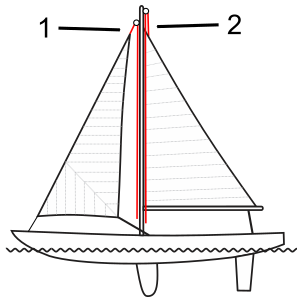
\includegraphics[width=\linewidth]{img/Halyard}
  \caption{1907 Franklin Model D roadster. Photograph by Harris \&
    Ewing, Inc. [Public domain], via Wikimedia
    Commons. (\url{https://goo.gl/VLCRBB}).}
  \Description{A woman and a girl in white dresses sit in an open car.}
\end{figure}

so important, please see
\url{https://www.acm.org/publications/taps/describing-figures/}.

\section{Citations and Bibliographies}

\begin{acks}
    Thanks is due to Dr. Kimball Germane of Brigham Young University, Provo,
    Utah for previewing drafts and offering feedback.
\end{acks}

\bibliography{\jobname}
\bibliographystyle{ACM-Reference-Format}

\end{document}
\endinput
%%
%% End of file `sample-sigconf-authordraft.tex'.
